\chapter{序論}
\label{introduction}

\section{背景}
\label{introduction:background}

2015年12月4日、Apple社が予てより同社の提供するCocoaおよびCocoa Touchフレームワークを用いたソフトウェアの開発用として提供していたプログラミング言語Swiftをオープンソース化し、Linuxを中心としたさまざまなプラットフォームにおけるソフトウェアを開発するための拡張を開始した。
これによりプログラミング言語SwiftはObjective-Cの担ってきたiOSやMac OS Xなどにおけるソフトウェアの開発だけでなく、C++やJavaなど他の汎用プログラミング言語が担ってきたソフトウェア開発においても、それらの代替となり得る可能性を持つこととなった。

Swiftはオブジェクト指向や全称型・存在型の導入、関数の第一級オブジェクト化、HindlyとMilnerによる型再構築アルゴリズムの採用など、現在多くのプログラマに使用されている他の汎用高級言語が持つ様々な特徴を持っているが、まだその特徴を採用するか否かがよく議論されていないものもある。
その内の1つがコンパイラをそのコンパイル対象の言語自体で開発するBootstrapプロセスの採用である。

表~\ref{table:bootstrapping-languages}はWeb検索エンジンにおけるクエリヒット数からプログラミング言語の知名度を格付けしたTIOBE Indexの2015年12月版において上げられている言語の内、汎用言語であるものだけを上位から20言語抽出し、それらの主要なコンパイラがその言語自体で記述されているかを示したものである。
この20言語の内だけでもBootstrapを行っているものが8言語あり、 その中に性能の問題からコンパイラ用の言語として採用されづらいインタプリタ型言語なども含まれていることを考慮すれば、かなりの言語がBootstrapされていることが分かる。
しかし、現在SwiftはC++を用いて開発されており、Bootstrapは行われていない。

現在Swiftにおいては未だ多くの機能が不足しており、他の問題を優先しているためにBootstrapについて大きく取り上げられてはいない。
また、開発者のメーリングリスト~\cite{dev-ml}では特にSwiftコンパイラのバックエンドとして採用されているLLVMのAPIがC++で提供されていることから、SwiftがC++と同様の役割を果たすにはもう少し時間が必要だという意見も上がっている。


しかし、~\ref{explain-bootstrap:merit}節で述べるようにBootstrapを行うことで得られる利益があることが他の言語の事例によって示されている以上、十分な議論なしに現状のSwiftにBootstrapが不要であると判断するのは早計であるといえる。

\begin{table}[tb]
    \begin{center}
        \caption{知名度の高いプログラミング言語のBootstrap状況}
        \begin{tabular}{|c|c|c|c|}
            \hline
            順位 & 言語名 & コンパイラ名 & Bootstrap状況 \\
            \hline
            1 & Java & javac & N (C, C++?) \\
            \hline
            1 & Java & OpenJDK & N (C++, Java) \\
            \hline
            2 & C & gcc & N (C++) \\
            \hline
            2 & C & clang & N (C++) \\
            \hline
            3 & C++ & gcc & Y \\
            \hline
            3 & C++ & clang & Y \\
            \hline
            3 & C++ & Microsoft Visual C++ & Y \\
            \hline
            4 & Python & cpython & N (C) \\
            \hline
            4 & Python & PyPy & Y \\
            \hline
            5 & C\# & Microsoft Visual C\# & N (C++) \\
            \hline
            5 & C\# & .NET Compiler Platform (Roslyn) & Y \\
            \hline
            6 & PHP & Zend Engine & N (C) \\
            \hline
            7 & Visual Basic .NET & Visual Studio & N (C++, C\#) \\
            \hline
            7 & Visual Basic .NET & .NET Compiler Platform (Roslyn) & Y \\
            \hline
            8 & JavaScript & SpiderMonkey & N (C, C++) \\
            \hline
            8 & JavaScript & V8 & N (C++, JavaScript) \\
            \hline
            9 & Perl & perl & N (C) \\
            \hline
            10 & Ruby & Ruby MRI & N (C) \\
            \hline
            12 & Visual Basic & Visual Studio & N (C++, C\#) \\
            \hline
            13 & Delphi/Object Pascal & Delphi & N (?) \\
            \hline
            13 & Delphi/Object Pascal & Free Pascal & Y \\
            \hline
            14 & Swift & swift & N (C++) \\
            \hline
            15 & Objective-C & clang & N (C++) \\
            \hline
            15 & Objective-C & gcc & N (C++) \\
            \hline
            17 & Pascal & Free Pascal & Y \\
            \hline
            17 & Pascal & GNU Pascal & N (C, Pascal) \\
            \hline
            20 & COBOL & GnuCOBOL & N (C, C++) \\
            \hline
            21 & Ada & GNAT & Y \\
            \hline
            22 & Fortran & GNU Fortran & N (C, C++) \\
            \hline
            22 & Fortran & Absoft Fortran Compiler & ? \\
            \hline
            23 & D & DMD & Y \\
            \hline
            24 & Groovy & groovy & N (Java, Groovy) \\
            \hline
        \end{tabular}
        \label{table:bootstrapping-languages}
    \end{center}
\end{table}

% \begin{figure}
%     \begin{center}
%         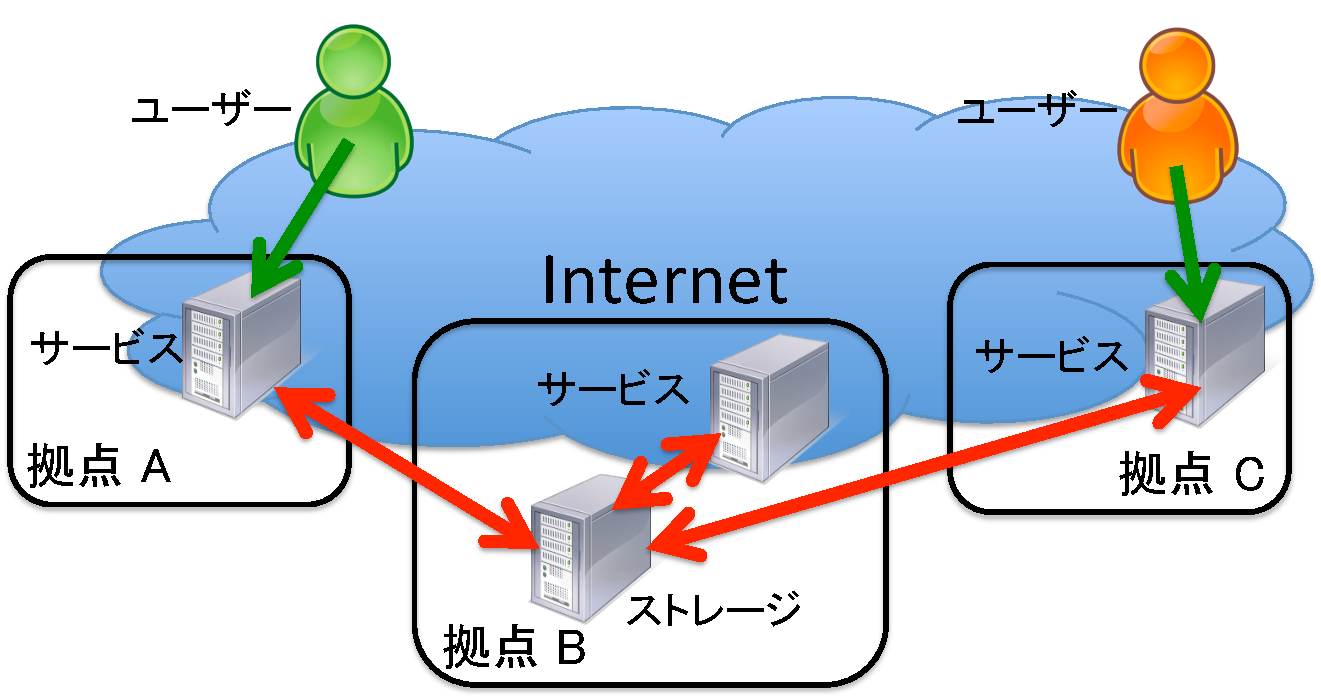
\includegraphics[scale=0.50]{./img/serviceanduser}
%         \caption{複数の拠点から提供されるサービス}
%         \label{img:mlservice}
%     \end{center}
% \end{figure}


\section{本研究が着目する課題}
\label{introduction:issue}

Swiftコンパイラが抱える他の問題との優先度や使用しているフレームワークとのつなぎ込みに関する問題が解決したとしても、SwiftコンパイラのBootstrapを行うかどうかという判断を下すにはより根源的な課題がある。
それは、現在Swiftを記述しているC++言語がSwiftと比較しても高い表現力を持っているために、~\ref{explain-bootstrap:instance}節で見る幾つかの事例とは異なり、Bootstrapを行うことで得られるメリットや、そもそも現行のコンパイラで使用されている手法を維持したままBootstrapを行うことが可能であるか否かが自明でないというものである。

また、現在のSwiftはC++との相互運用性を持っていないため、コンパイラ中の一部分をSwiftで記述したものに置き換えることは難しく、逆に実際に使用されているコンパイラ中のモジュール化が可能なほど大きなパーツをSwiftへ移植するとなると、その間の言語への機能追加などの改変は現行のものと移植中のものの両者に適用するか、移植中のもののみに追加して移植が完了するまでその適用を先送りしなくてはならなくなってしまう。


\section{本研究の目的}
\label{introduction:purpose}

本研究では、SwiftコンパイラがBootstrapすることによって得られるメリットと被るデメリットを定量的に示し、Bootstrapを行うべきか否かを判断する上で有用な情報を収集することを目的とする。
そのためのアプローチとして、Swiftコンパイラの基幹的機能である構文解析器をSwiftによって実装し、その実行時間とソースコードの行数を現行のSwiftコンパイラの構文解析器と比較する。
また、この独自の構文解析器は現行のSwiftコンパイラと基本的な設計手法において同じものを採用するだけで、完全に独立させたものとして実装する。

この方法により、現在のSwiftコンパイラの開発状況などの影響を一切受けずにBootstrapのための評価が可能となり、またその評価がBootstrapの可能性に対して有意義な知見を与えることを提示する。


\section{本論文の構成}

本論文の構成は次の通りである。

第2章では本研究の考察対象であるコンパイラのBootstrapについてSwift以外の言語の事例からそのメリットについてまとめ、Bootstrapにおける課題について整理する。
第3章では本研究が着目するプログラミング言語Swiftの特徴とそのコンパイラ実装の基幹部分における特徴について説明する。
第4章では現行のSwiftコンパイラとの比較対象となるSwiftで記述したSwiftコンパイラ「TreeSwift」の構成について述べ、現行のコンパイラとその基本的な設計手法などに大きな差異がないことを確認する。
第5章では現行のSwiftコンパイラとTreeSwiftの構文解析器についてその実行速度とソースコードの行数を比較し、その結果について考察する。
第6章では本研究の結論と今後の展望についてまとめる。

%%% Local Variables:
%%% mode: japanese-latex
%%% TeX-master: "../thesis"
%%% End:
